\chapter{The OpenCL Programming Model}
\label{ch4_opencl}

OpenCL is a framework for writing application programs that run across heterogeneous platforms, comprising \ac{GPU}, \ac{CPU}, \ac{DSP}, \ac{FPGA}, and other processors or hardware accelerators \cite{opencl_wiki}. A framework suited for parallel programming, it has been standardized by the Khronos group, which includes companies like AMD, Apple, Intel, NVIDIA, Qualcomm, Sony, Xilinx, etc.\cite{opencl_fixstars}.

\section{Introduction}
\label{sect4_1}

OpenCL is truly the first open programming standard for general-purpose computations on heterogeneous systems, allowing programmers to target their source code on multi-core CPUs, GPUs, and other devices. It specifies a programming language (centered on the C99 standard) for programming these devices and provides \ac{API}s, to control the platform and execute programs on heterogeneous computing devices. OpenCL is vendor independent and thus not specialized for any device. Therefore, OpenCL is a powerful way to write parallel programs capable of running on a wide range of devices. \newline\newline
The framework includes a language, API, libraries and a runtime system to support software development. The architecture of OpenCL can be described using a hierarchy of models \cite{opencl_ajg}:

\begin{itemize}
\item Platform Model
\item Memory Model
\item Execution Model
\item Programming Model
\end{itemize}

\subsection{Platform Model}
\label{sect4_1_1}
In this model, a host device is connected to one or more OpenCL devices, which is divided into one or more compute units (CUs), further divided into one or more processing elements (PEs). All computations on a device are executed on the PEs \cite{opencl_khronos}.

\begin{figure}[h!]
  \centering
  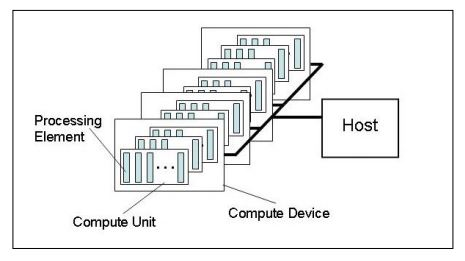
\includegraphics[width=10cm]{figures/OpenCL_Platform_Model.JPG}
  \caption{Platform Model in OpenCL}
  \label{fig:opencl1}
\end{figure}
The host device holds the OpenCL application running, from where the commands are submitted to the device, to be executed on the PEs within. The PEs inside a CU execute a single set of instructions as Single Instruction Multiple Data (SIMD) units in parallel. 

\subsection{Memory Model}
\label{sect4_1_2}
Memory directly available to kernels executing on OpenCL devices is known as device memory. The device memory consists of the four distinct memory regions as follows: 
\begin{itemize}
\item \textbf{Global Memory}: This memory region allows read/write access to each work item in all the work groups executing on any device inside a context. Work items are capable of reading from or writing to any part of memory objects. Accesses to global memory may be cached, depending on the device capabilities. \newline\newline
Global memory is shared with all processing elements, and is also available to the host. The host utilises this memory to copy data to/from the device.

\item \textbf{Constant Memory}: This memory region contains content that remains constant throughout the execution of a kernel. \newline\newline
Constant memory is also shared between all processing elements, but it is read-only. It provides an efficient way to share data with all processing elements.

\item \textbf{Local Memory}: A region of memory local to a work group. This region can be used to allot variables that are common to all work items within the work group.\newline\newline
Each CU has its own local memory, only shared with the processing elements within the compute unit. It cannot be accessed by other compute units. 

\item \textbf{Private Memory}: A region of memory private to a work item. Variables declared in one work item’s private memory are not visible to another work item.\newline\newline
Private memory belongs to a single processing element. Each processing element has its own private memory, thereby unable to access all other private memories within or outside the CU.

\begin{figure}[h!]
 \centering
  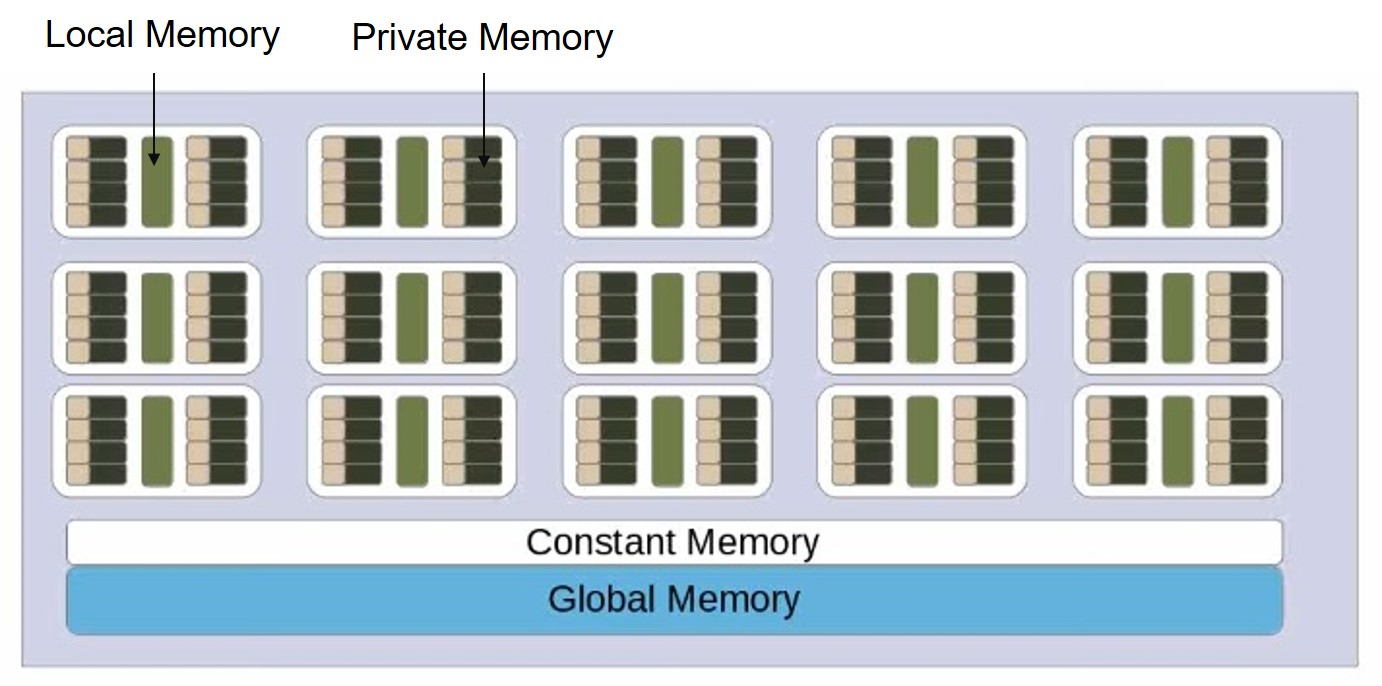
\includegraphics[width=\linewidth]{figures/OpenCL_Memory_Model.jpg}
  \caption{Memory Model in OpenCL \cite{opencl_ajg}}
  \label{fig:opencl2}
\end{figure}
\end{itemize}
Global memory is the only memory which is persistent between kernel calls. Constant, local, and private memories are just scratch spaces, which get reset after every kernel call.

 \subsection{Execution Model}
 \label{sect4_1_3}
The core of the OpenCL execution model is based on how kernels execute on the device. The execution of an OpenCL program happens in two parts: kernels that execute on the OpenCL devices, and a host that runs on the host device. The host is responsible for executing kernel functions on the device \cite{opencl_khronos}. These are ordinary functions, albeit with special signatures. The kernel call comprises two parts: an ordinary argument list, and external execution parameters that control the parallelism. OpenCL provides direct support for parallel computing. \newline\newline
\begin{figure}[h!]
\centering
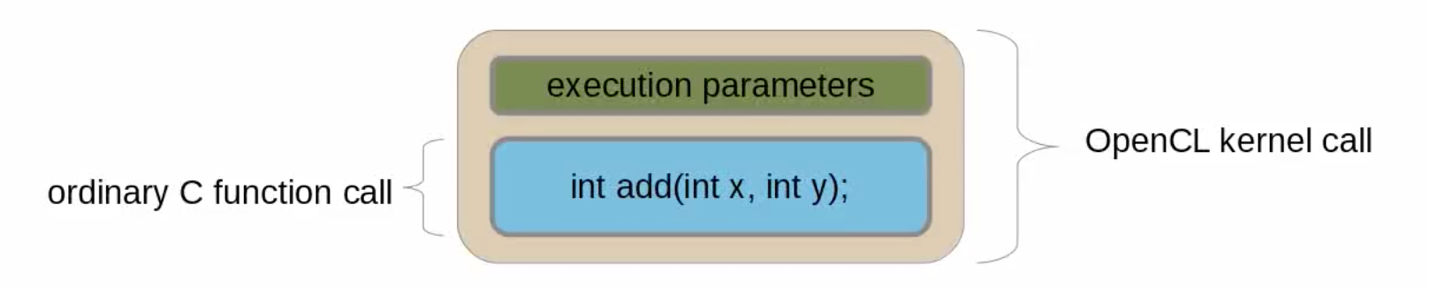
\includegraphics[width=\linewidth]{figures/C_and_OpenCL_Function_Calls.png}
\caption{C and OpenCL Function Calls \cite{opencl_ajg}}
\label{fig:opencl3}
\end{figure}
The host coordinates the execution of the kernels on the OpenCL device. It does not get involved in the computations itself; it only provides execution parameters to launch the kernel and the arguments which the kernel requires for carrying out the operations. 

\subsubsection{Execution Strategy}
\label{sect4_1_3_1}
The kernel function will be invoked many times, the argument list being identical for all the invocations. This means that the same function gets called repeatedly, based on the execution parameters specified by the host prior to launching the kernel.\newline\newline
There exists an index space provided by an N-dimensional index space. The index space supported in OpenCL is called an NDRange. It can be one, two or three dimensional. Each function invocation can access its index; this is how it is identified. A work item is a kernel invocation for a particular index, and the global id is a unique identity for every work item belonging to the index space. Every work item is provided with a global ID. The global work size is the number of work items in every dimension. The work dimension is the dimension of the index space.\newline\newline 
From the Device Model, the processing elements are the ones which execute the instructions. To be able to execute the kernel multiple times on the device, the work item needs to be mapped to Processing Elements (PEs). Multiple work items are assigned to each PE, so that the case where number of PEs is less than the global work size can be taken care of. \newline\newline
Now, every Compute Unit (CU) has a dedicated local memory which is shared by all PEs within. Local memory provides huge advantages in performance. Thus, work items must be mapped to the PEs in such a way that a group of them can access the local memory of a CU for effective execution. The partitioning of the global work size into smaller pieces leads to the formation of work groups. The work groups provide a more coarse-grained decomposition of the index space. Work groups are assigned a unique work group ID with the same dimension as the index space used for the work items. Work items are assigned a unique local ID within a work group so that a single work item can be uniquely identified by its global ID or by a combination of its local ID and work group ID \cite{opencl_khronos}. \newline\newline
Work groups execute on CUs and share their local memory. All the work items in the work group share local memory and are mapped to PEs within a CU. These work items are capable of identifying which work group they are parts of, work group ID, size of work groups, their global IDs and the global work size. \newline\newline 
The work group size has a device-specific physical meaning. The maximum work group size is a device characteristic. This can be determined by querying the device. Also, it is an integer value; thus, n-dimensional work groups have to be handled in a special way. Work groups are launched by the host device. \newline\newline
The device dependent work group size is a scalar, but work groups can have multiple dimensions. For example, if the maximum work group size is 32, work groups could be launched in 3 dimensions like (8, 2, 2). The following must be true in order to launch the work groups successfully: 
\begin{figure}[h!]
\centering
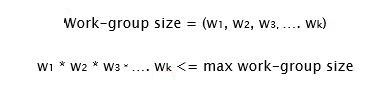
\includegraphics[width=\linewidth]{figures/Work-Group_Size.JPG}
\caption{Handling multi-dimensional work group sizes}
\label{fig:opencl4}
\end{figure} 

The figure below shows an example of how the local size, number of work groups and global size vary for different dimensions of \verb|NDRange|:
\begin{figure}[h!]
\centering
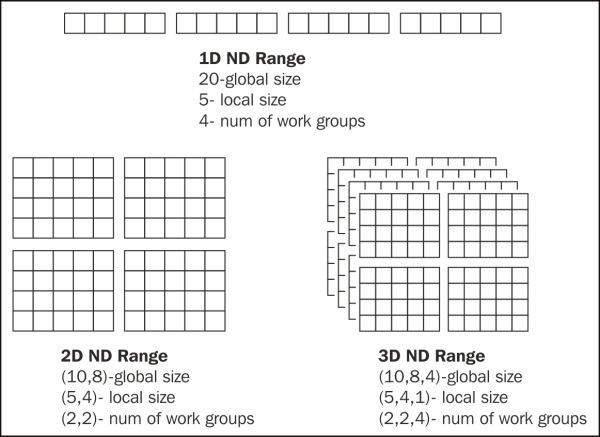
\includegraphics[width=\linewidth]{figures/NDRange_Kernel_Example.jpg}
\caption{NDRange multi-dimensional index space example}
\label{fig:opencl5}
\end{figure}

\subsubsection{Host API}
\label{sect4_1_3_2}
The host must call certain APIs in order to execute the kernels, which take care of the following:
\begin{itemize}
\item Platform \newline
A platform is an implementation of OpenCL. These are the drivers for specific devices which support the execution of OpenCL kernels. Platforms enables supported devices to be exposed to the programmer. For example, if a system consists of 1 AMD GPU, 1 NVIDIA GPU and an Intel Xeon Phi CPU, all capable of running OpenCL code, there will be three platforms corresponding to each of these devices. The platform is used to discover devices available.
\item Context \newline
A context is created by the host for each platform on which the kernel executes. Thus, a context cannot have multiple platforms. A context acts as a container for devices and memory. Most kernel operations are related to a context.
\item Program \newline
A program is a collection of kernels. A program is loaded by the host device and kernels are extracted from the program to be invoked. The host could either directly compile the OpenCL C code or load a binary representation. Programs are device specific.
\item Asynchronous Device Calls \newline
The host manages devices asynchronously. Host issues commands to the device, telling the device to perform some work. Devices act as slaves and do as the instructed command. The host waits for the commands to complete, meaning that the device has completed the action. Commands can have dependencies on other commands. OpenCL commands are issued by \verb|clEnqueue*| calls. A \verb|cl_event| returned by \verb|clEnqueue*| calls is used for dependencies.

\end{itemize}

 \subsection{Programming Model}
 \label{sect4_1_4}
The OpenCL execution model supports data parallel and task parallel programming models. In OpenCL, the primary model is data parallel. \newline

\subsubsection{Data Parallel}
\label{sect4_1_4_1}
Data parallel programming model (equivalent to SIMD) defines computations in terms of a sequence of instructions applied to multiple elements of a dataset. In a strict data parallel model, a one-to-one mapping exists between a work item and an element in the dataset over which a kernel can be executed in parallel. However, a strict one-to-one mapping is not required in OpenCL. \newline\newline
A hierarchical data programming model exists in OpenCL, where the hierarchical subdivision can be achieved either explicitly or implicitly. In the explicit model, the total number of work items to execute in parallel and how work items are divided among work groups must be defined by the programmer. On the other hand, the implicit model only requires the total number of work items to execute in parallel to be defined, while the division into work groups is taken care by the OpenCL implementation.

\subsubsection{Task Parallel}
\label{sect4_1_4_2}
Task parallel programming model in OpenCL defines a model in which a single instance of a kernel is executed independent of any index space. It is equivalent to executing a kernel on a compute unit with a work group containing a single work item. It is the simultaneous execution of many different tasks across the same or different memory objects.

\section{Experiments}
\label{sect4_2}
A few simple experiments were conducted on different devices – an AMD GPU and an NVIDIA GPU, to see how performance varied on using the same OpenCL kernel code but with different execution parameters. A small kernel which performs 2-dimensional matrix multiplication was written in OpenCL and was launched with different global sizes and work group sizes on the specific platform to see how  execution timings varied. \newline\newline
The host device selects the platform and the device, creates the context and command queue, initializes the matrices, creates memory buffers in the device, and transfers the data to the device memory. The two input matrices and one output matrix are passed to the kernel function as arguments, on which the matrix multiplication was performed in parallel. The execution is controlled by the \verb|clEnqueueNDRangeKernel| parameters, which define the work group size by specifying the local size and global size. \newline\newline

\begin{equation}
\mathbf{Work\, group\, size = Local\, size}
\end{equation}

The number of work groups can be found out as follows:
\[Number \, of \, work \, groups=\frac{Global \, Size \,}{Local \, Size}\]

The work group size must be perfectly divisible by the specified global work size, failing which the kernel would not be launched and an error would be thrown. A work group gets mapped to a compute unit for execution. \newline\newline
The global size, or index space depends on the total number of computations required to be performed. In matrix multiplication, this value is the dimension of the matrices. For example, if two 4 x 4 matrices are to be multiplied, the global size would be two-dimensional, represented as (4,4). \newline\newline
The matrix resultant as the product of the two input matrices was stored in a buffer and transferred back to the host asynchronously. The execution time was calculated and the result was compared for correctness by running the matrix multiplication sequentially on the host device.\newline\newline
In the experiments conducted, the sizes of the matrices \textit{(or global size)} being multiplied was increased from 128 to 2048, and for each global size, the work group size was changed from 2 to 128. The objective of these experiments was to notice the effect of changing the mapping of work groups onto the compute units of the device on the kernel execution timings.

\subsection{Results}
\label{sect4_2_1}
The following tables show the average timing results on AMD Radeon HD 8730M on platform OpenCL 2.0 AMD-APP (1800.8) and NVIDIA GeForce 405 on OpenCL 1.1 CUDA 4.2.1.
\begin{table}[h!]
\centering
 \caption{Execution time (in µs) of matrix multiplication on AMD Radeon HD 8730M GPU}
 \vspace{3mm}
 \renewcommand\arraystretch{1.2}
 \begin{tabular}{|l|*{5}{r|}}
 \hline
 \multicolumn{6}{|c|}{2-D Matrix Multiplication: Timings on AMD GPU} \\
 \hline
 \backslashbox{\bfseries{Local}}{\bfseries{Global}}
 &\makebox[4.5em]{\bfseries{128}}&\makebox[4.5em]{\bfseries{256}}&\makebox[4.5em]{\bfseries{512}}
&\makebox[4.5em]{\bfseries{1024}}&\makebox[5.5em]{\bfseries{2048}}\\
 \hline
 Not Specified & 6121.25 & 48282.5 & 401073.58 & 3270198.86 & 16901530.39\\	
 2 & 8400.23 & 67250.57 & 530250.24 & 1082663.32 & 5365565.08\\
 4 & 2181.05 & 16945.09 & 142875.45 & 298480.89 & 1703353.98\\
 8 & 3359.17 & 25594.24 & 206148.51 & 265741.50 & 1362683.18 \\
 16 & 6123.93 & 48253.26 & 385895.55 & 291104.51 & 1243956.77\\
 32 & \textit{Error} & \textit{Error} & \textit{Error} & \textit{Error} & \textit{Error}\\
 64 & \textit{Error} & \textit{Error} & \textit{Error} & \textit{Error} & \textit{Error}\\
 128 & \textit{Error} & \textit{Error} & \textit{Error} & \textit{Error} & \textit{Error}\\
 \hline
 \end{tabular}
 \label{table:matrix2D_AMD}
\end{table} \newline

\begin{table}[h!]
\centering
 \caption{Execution time (in µs) of matrix multiplication on NVIDIA GeForce 405 GPU}
 \vspace{3mm}
 \renewcommand\arraystretch{1.2}
 \begin{tabular}{|l|*{4}{r|}{c|}}
 \hline
 \multicolumn{6}{|c|}{2-D Matrix Multiplication: Timings on NVIDIA GPU} \\
 \hline
 \backslashbox{\bfseries{Local}}{\bfseries{Global}}
 &\makebox[4.5em]{\bfseries{128}}&\makebox[4.5em]{\bfseries{256}}&\makebox[4.5em]{\bfseries{512}}
&\makebox[4.5em]{\bfseries{1024}}&\makebox[5.5em]{\bfseries{2048}}\\
 \hline
 Not Specified & 6138.05 & 48312.10 & 401356.14 & 5773783.80 & \textit{Error}\\	
 2 & 10721.54 & 58040.95 & 621084.80 & 4527345.84 & \textit{Error}\\
 4 & 3488.40 & 18654.32 & 232133.67 & 1776133.69 & \textit{Error}\\
 8 & 2969.30 & 17499.01 & 229669.94 & 1729808.40 & \textit{Error} \\
 16 & 8382.89 & 34673.16 & 486371.19 & 3369363.59 & \textit{Error}\\
 32 & \textit{Error} & \textit{Error} & \textit{Error} & \textit{Error} & \textit{Error}\\
 64 & \textit{Error} & \textit{Error} & \textit{Error} & \textit{Error} & \textit{Error}\\
 128 & \textit{Error} & \textit{Error} & \textit{Error} & \textit{Error} & \textit{Error}\\
 \hline
 \end{tabular}
 \label{table:matrix2D_NVIDIA}
\end{table}

\subsection{Discussion}
\label{sect4_2_2}
Table \ref{table:matrix2D_AMD} and Table \ref{table:matrix2D_NVIDIA} show the execution time (in µs) taken by the two-dimensional matrix multiplication kernel in OpenCL on AMD and NVIDIA GPUs, for different local sizes. The matrix sizes were increased from 128 x 128 to 2048 x 2048 and the execution times were measured and noted. \newline\newline
The results can be analysed better by comparing the performance of both devices in \ac{GOPS} for different global sizes, calculated in Table \ref{table:matrix2D_gops}. It has been computed by dividing the number of operations by the best performing OpenCL execution timings among the different local sizes, specified in Tables \ref{table:matrix2D_AMD} and \ref{table:matrix2D_NVIDIA}. The performance in GOPS for AMD Radeon 8730M and NVIDIA GeForce 405 are for local sizes 4 and 8, respectively.

\begin{table}[h!]
\centering
 \caption{Performance in GOPS for AMD Radeon 8730M and NVIDIA GeForce 405 for different global sizes}
 \vspace{3mm}
 \renewcommand\arraystretch{1.4}
 \begin{tabular}{|l|*{2}{c|}}
 \hline
 \multicolumn{3}{|c|}{2-D Matrix Multiplication: Performance in GOPS} \\
 \hline
 \backslashbox{\bfseries{Size}}{\bfseries{Device}}
 &\makebox[4.5em]{\bfseries{AMD}}&\makebox[4.5em]{\bfseries{NVIDIA}}\\
 \hline
 128 & 5.78 & 4.25 \\ 
 256 & 5.95 & 5.76 \\
 512 & 5.64 & 3.51 \\
 1024 & 21.59 & 3.73 \\
 2048 & 30.26 & \textit{Not Applicable} \\
 \hline
 \end{tabular}
 \label{table:matrix2D_gops}
\end{table}

As seen in Figure \ref{fig:opencl6}, the number of operations performed during the execution is equal to \verb|6 * GLOBAL_SIZE|\textsuperscript{3} \verb|+ 2 * GLOBAL_SIZE|\textsuperscript{2} where the \verb|GLOBAL_SIZE| varies from 128 to 4096 as exponents of 2. This program has a code complexity of O(\(n^3\)) which largely increases the number of operations.
\begin{figure}[h!]
\centering
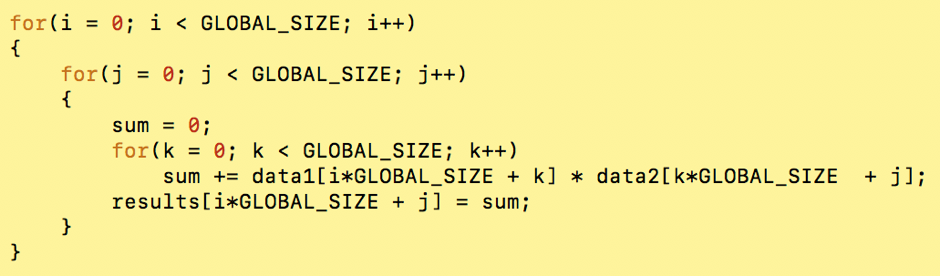
\includegraphics[width=\linewidth]{figures/Matrix_Multiplication_2D.png}
\caption{Code for matrix multiplication in 2D}
\label{fig:opencl6}
\end{figure}

As observed in the results, the AMD Radeon 8730M overpowers the NVIDIA GeForce 405 if their best execution times are compared for different global sizes. Both the devices follow a similar trend for maximum performance (or least execution time). For both the devices, there exists a trend of having a least execution time at a particular work group size, beyond which the increasing the local work size leads to higher execution times (lower performance). In the case of AMD Radeon 8730M, the best performance is achieved when the work group size is 4, while for NVIDIA GeForce 405 it is 8. The best performing work group size values are device specific, as seen from the results. \newline\newline
Upon further increasing the work group size, it was noticed that the execution of OpenCL kernel was failing due to error in launching it. This work group size was 32 for both AMD Radeon 8730M and NVIDIA GeForce 405. This falls in line with the Section 4.1.3.1 Execution Strategy, which mentions that the maximum work group size is device-specific. Thus, we can conclude that the maximum work group size for both the GPUs is 16. \newline
